\chaplbl{Expertise and Memory}{sec:memory}

Returning to educational psychology, we now discuss what distinguishes
expertise from earlier stages of learning, how expertise can be helpful
and harmful, and then describe concept maps, a tool that can help expose
expertise.

\seclbl{Connectivity}{sec:connectivity}

\secref{sec:novice} described
the key difference between novices and competent practitioners. What
makes experts different from either? The answer is not that they know
more facts: competent practitioners can memorize a lot of trivia without
any noticeable improvement to their performance.

To explain the difference, imagine for a moment that we store knowledge
as a graph in which facts are nodes and relationships are arcs. (This is
emphatically \emph{not} how our brains work, but it's a useful
metaphor.) The key difference between experts and people who are
``merely competent'' is that experts have many more connections, i.e.,
their mental models are much more densely connected.

To understand expert behavior, think about driving around a city,
comparing what it's like for the local and for the out-of-town driver.

This metaphor helps explain many observed aspects of expert behavior:

\begin{enumerate}
\item
  Experts can jump directly from a problem to its solution because there
  actually is a direct link between the two in their mind: where a
  competent practitioner would have to reason ``A, B, C, D, E'', the
  expert can go from A to E in a single step. We call this
  \emph{intuition}, and it isn't always a good thing: when asked to
  explain her reasoning, an expert often can't because she didn't
  actually go through any intermediate steps.

  \emph{In our example above, the local probably doesn't even think
  about which turns they're making on their way to the grocery store.
  They can drive on ``autopilot'' without really thinking. If someone
  asks them to go to a different location, they immediately know what
  they should do next to get to the right place.}
\item
  Experts are frequently so familiar with their subject that they can no
  longer imagine what it's like to \emph{not} see the world that way. As
  a result, they are often less good at teaching the subject than people
  with less expertise who still remember what it's like to have to learn
  the things. This is called \emph{expert blind spot}. It can be
  overcome with training, but it's part of why world-famous researchers
  are often poor lecturers.

  \emph{The local driver will forget to tell the out-of-towner that the
  bridge is under construction, or that there's always a train at 3:00,
  because it has been like that for years. The local driver will tell
  the out-of-towner to turn ``where the gas station used to be''.}
\item
  Densely-connected knowledge graphs also explains \emph{fluid
  representations}, e.g., expert mathematicians' ability to switch
  effortlessly between algebraic and geometric views of a problem.

  \emph{The local driver probably can use either the names of streets}
  or \emph{landmarks when giving directions. The out-of-towner only has
  street labels.}
\item
  Finally, this metaphor also explains why experts are better at
  diagnosis than competent practitioners: more linkages between facts
  makes it easier to reason backward from symptoms to causes. (And this
  in turn is why asking programmers to debug during job interviews gives
  a more accurate impression of their ability than asking them to
  program.)

  \emph{When the out-of-towner finally calls their local friend, saying
  ``well, we just passed Sycamore Street and we can see a restaurant
  named Nellie's Cafe'', the local can more easily figure out where the
  out-of-towner is, and how to get to their destination.}
\end{enumerate}

\begin{callout}{The J Word}{callout:the-j-word}

Experts often betray their blind spot by using the word ``just'' in
explanations, as in, ``Oh, it's easy, you just fire up a new virtual
machine and then you just install these four patches to Ubuntu and then
you just re-write your entire program in a pure functional style---no
problem.'' As we discuss later in \secref{sec:motivation},
the J word (also sometimes called the passive dismissive
adjective) is banned in our workshops, primarily because using it gives
learners the very clear signal that the instructor thinks their problem
is trivial and that they therefore must be stupid.
\end{callout}

The graph model of knowledge explains why helping learners make
connections is as important as introducing them to facts. The more
people you know in a group, the more likely you are to remain part of
that group. Similarly, the more connections a fact has to other facts,
the more likely the fact is to be remembered. This builds on our earlier
idea of mental models - a mental model is a way to facilitate making
connections between separate facts.

\begin{callout}{Repetition vs.~Reflective Practice}{callout:repetition-vs.reflective-practice}

The idea that ten thousand hours of practice will make someone an expert
in some field is widely known, but reality is much more complex. First,
practice is not doing the same thing over and over again: practice is
doing similar but subtly different things, getting feedback, and then
changing behavior in response to that feedback to get cumulatively
better. Doing the same thing over and over again is much more likely to
solidify bad habits than perfect performance.

Second, a \href{http://pss.sagepub.com/content/25/8/1608}{meta-study in
2014} found that ``\ldots{}deliberate practice explained 26\% of the
variance in performance for games, 21\% for music, 18\% for sports, 4\%
for education, and less than 1\% for professions.'' One explanation for
this variation is that deliberate practice works best when the rules for
evaluating success are very stable, but is less effective when there are
more factors at play.
\end{callout}

\seclbl{Concept Maps}{sec:concept-maps}

Our tool of choice to represent an expert's knowledge graph is the
\emph{concept map}. A concept map is simply a picture of someone's
mental model of a domain: facts are bubbles, and connections are
labelled arcs. It is important that they are labelled: saying ``X and Y
are related'' is only helpful if we explain what the relationship
\emph{is}. And yes, one person's fact may be another person's
connection, but by \emph{externalizing cognition} (i.e., making thought
processes and mental models visible), concept maps help spark and focus
discussion.

\begin{callout}{There's More Than One Way to Do It}{callout:theres-more-than-one-way-to-do-it}

Concept maps are just one way to represent our understanding of a
subject. Flowcharts, decision trees, and blueprints can be even more
useful in some contexts. For example,
\href{fixme-abela}{this diagram}
(taken from \href{http://extremepresentation.typepad.com/blog/2006/09/choosing\_a\_good.html}{a blog post}
by Andrew Abela) is an excellent way to organize and present
an understanding of how to choose the right kinds of chart for
displaying different kinds of data.
\end{callout}

To show what concept maps look like, consider this simple \texttt{for}
loop in Python:

\begin{verbatim}
for ch in "abc":
    print(2*ch)
\end{verbatim}

The three key concepts used in this loop are:

\begin{figure}[htbp]
\centering
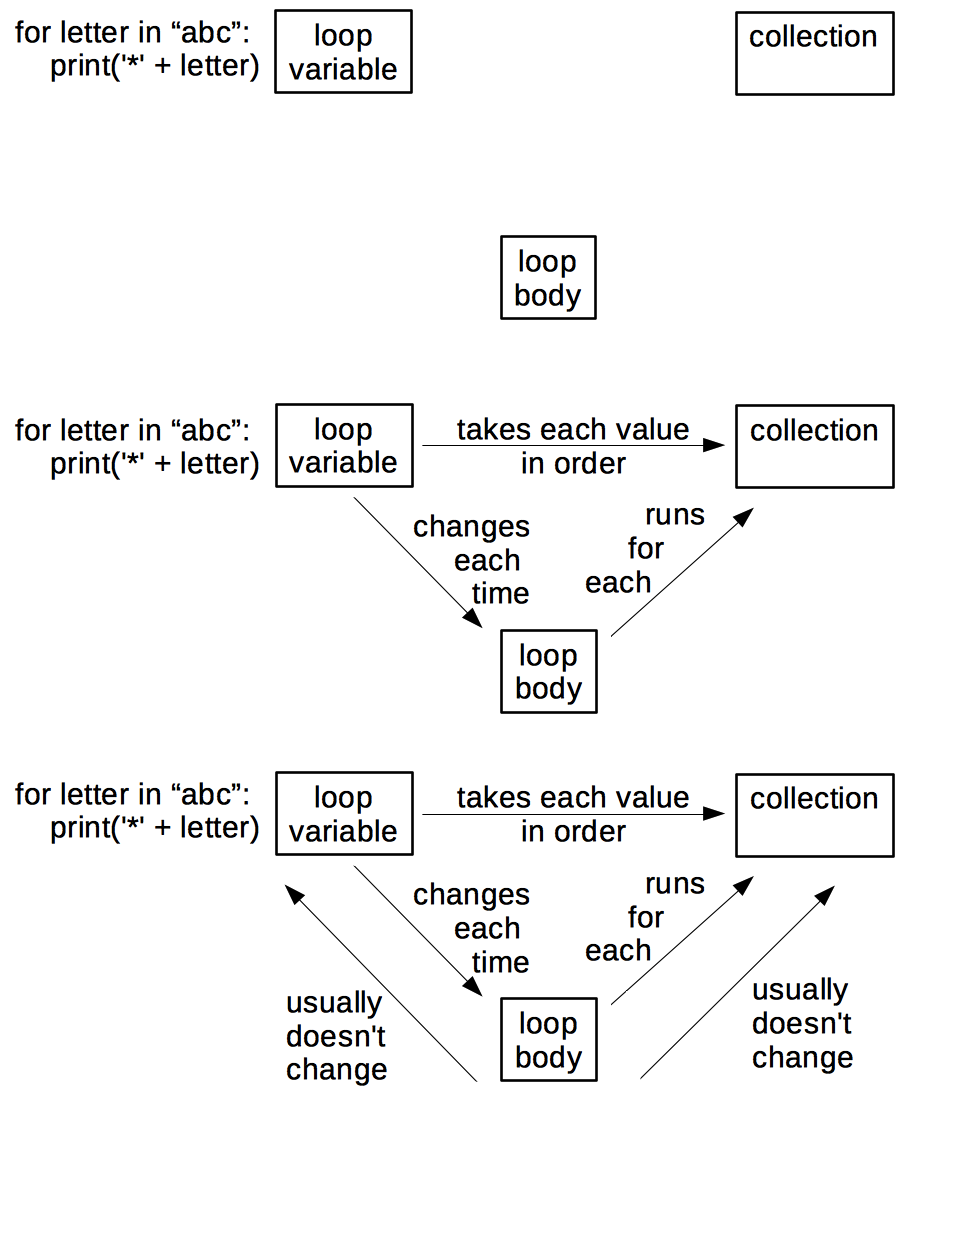
\includegraphics{../fig/for-loop-concepts.png}
\caption{Key Concepts}
\end{figure}

(In this case it's easy to connect the concepts to concrete elements in
the program, but that may not always be the case.) The key
relationships, which are as important as the concepts themselves, are:

\begin{figure}[htbp]
\centering
\includegraphics{../fig/for-loop-arcs.png}
\caption{Relationships}
\end{figure}

A quick count shows that there are actually 6 things here, not just 3,
so we're already brushing up against the limits of short-term memory. If
we add two more facts to show things that are usually (but not always)
true:

\begin{figure}[htbp]
\centering
\includegraphics{../fig/for-loop-rec.png}
\caption{Recommendations}
\end{figure}

the count rises to 8, which is a good size for a single teaching
episode. A few other concept maps drawn by previous participants in this
training course are listed below:

\begin{itemize}
\item
  \href{../fig/array-math.png}{Array Math}
\item
  \href{../fig/conditionals.png}{Conditionals}
\item
  \href{../fig/create-destroy.png}{Creating and Destroying Files}
\item
  \href{../fig/dict-set.png}{Sets and Dictionaries in Python}
\item
  \href{../fig/io.png}{Input and Output}
\item
  \href{../fig/lists-loops.png}{Lists and Loops}
\end{itemize}

Most of these are larger than our recommended limit, but that's not
necessarily a bad thing: after drawing a concept map for an entire
subject, a lesson designer can then carve out tightly-connected
sub-graphs to make individual episodes.

Concept maps can be used in many ways:

\begin{enumerate}
\item
  To aid solo design of a lesson by helping authors figure out what
  they're trying to teach. Crucially, a concept map separates content
  from order: in our experience, people rarely wind up teaching things
  in the order in which they first drew them.
\item
  They aid communication with fellow lesson designers. Instructors with
  very different ideas of what they're trying to teach are likely to
  pull their learners in different directions. Drawing and sharing
  concept maps isn't guaranteed to prevent this, but it certainly helps.
\item
  Concept maps also aid communication with learners. While it's possible
  to give learners a pre-drawn map at the start of a lesson for them to
  annotate, it's better to draw it piece by piece while teaching to
  reinforce the ties between what's in the map and what the instructor
  said. (We will return to this idea below when discussing Mayer's work
  on multimedia learning.)
\item
  Concept maps are also a useful formative assessment technique: having
  learners draw concept maps of what they think they just heard shows
  the instructor what was missed and what was mis-understood. Reviewing
  the learners' concept maps is too time-consuming for use in workshops,
  but very useful in weekly lectures \emph{once learners are familiar
  with the technique}: as
  \href{http://www.amazon.com/Facts-Fallacies-Software-Engineering-Robert/dp/0321117425/}{Glass
  observed}, any new tool or technique initially slows people down.
\end{enumerate}

Concept maps are also useful for many other kinds of tasks. For example,
the next time you have a team meeting, give everyone a sheet of paper
and have them spend a few minutes drawing a concept map of the project
you're all working on---separately. On the count of three, have everyone
reveal their concept maps simultaneously. The discussion that follows
everyone's realization of how different their mental models of the
project's aims and organization are is always interesting\ldots{}

Concept maps are also a useful way to organize one's thoughts before
putting together a talk or writing a paper. As with lessons, they allow
us to \emph{externalize cognition}, i.e., to get our thoughts out where
we can see them (and see the contradictions that have happily been
swimming around inside our heads without bumping into each other).

\begin{challenge}{Concept Mapping}{chal:concept-mapping}

Create a hand drawn concept map for something you would teach in five
minutes. (Possibly for the same subject that you used to create a
multiple choice question before.) Trade with a partner, and critique
each other's maps. Do they present concepts or surface detail? Which of
the relationships in your partner's map do you consider concepts and
vice versa?
\end{challenge}

\begin{callout}{Building Concept Maps Together}{callout:building-concept-maps-together}

Concept maps can be used as a classroom discussion exercise. Put
learners in small groups (2-4 people each), give each group some sticky
notes on which a few key concepts are written, and have them build a
concept map on a whiteboard by placing those sticky notes, connecting
them with labelled arcs, and adding any other concepts they think they
need.
\end{callout}

\begin{callout}{What Are We Doing Again?}{callout:what-are-we-doing-again}

Concept maps can also be used to help build a shared understanding of
what a project is trying to accomplish. Everyone independently draws a
concept map to show what they think the project's goals and constraints
are. Those concept maps are then revealed simultaneously. The ensuing
discussion can be\ldots{}vigorous.
\end{callout}

\seclbl{Seven Plus or Minus Two}{sec:seven-plus-or-minus-two}

\begin{challenge}{The Serial Position Effect}{chal:the-serial-position-effect}

Read the following list and try to memorize the items in it:

cat, apple, ball, tree, square, head, house, door, box, car, king,
hammer, milk, fish, book, tape, arrow, flower, key, shoe

Without looking at the list again, write down as many words from the
list as you can. Compare to other members of the group. What words are
remembered the most?

\href{http://cat.xula.edu/thinker/memory/working/serial}{This website}
implements an interactive version of this exercise.
\end{challenge}

While the graph model of knowledge is inaccurate but useful, another
simple model of knowledge has a sound physical basis. As a rough
approximation, human memory can be divided into two different storage
layers. The first is called \emph{long-term} or \emph{persistent
memory}. It is where we store things like our password, our home
address, and what the clown did at our eighth birthday party that scared
us so much. It is essentially unbounded (barring injury or disease, we
will die before it fills up) but it is slow to access---too slow to help
us handle hungry lions and disgruntled family members.

Evolution has therefore given us a second system called
\emph{short-term} or \emph{working memory}. It is much faster, but also
much smaller: in 1956, Miller estimated that the average adult's working
memory could hold
\href{https://en.wikipedia.org/wiki/The\_Magical\_Number\_Seven,\_Plus\_or\_Minus\_Two}{7±2
items} for a few seconds before things started to drop out. This is why
phone numbers are typically 7 or 8 digits long: back when phones had
dials instead of keypads, that was the longest string of numbers most
adults could remember accurately for as long as it took the dial to go
around and around. It's also why sports teams tend to have about half a
dozen members, or be broken down into smaller groups (such as the
forwards and backs in rugby).

When we memorize words in a list and are asked to immediately recall
them, the words first presented will have the best chance to be
transferred into long-term memory. On the other hand, the items that are
presented last might still be in short-term memory. These are referred
to as the primacy and recency effects, respectively, and they together
form the
\href{https://en.wikipedia.org/wiki/Serial\_position\_effect}{memory
serial position effect}.

\begin{callout}{Chunking}{callout:chunking}

Our minds can store larger numbers of facts in short-term memory by
creating \emph{chunks}. For example, most of us will remember a word we
read as a single item, rather than as a sequence of letters. Similarly,
the pattern made by five spots on cards or dice is remembered as a whole
rather than as five separate pieces of information. Chunks allow us to
manage larger problems, but can also mislead us if we mis-identify
something, i.e., see it as something it isn't.
\end{callout}

7±2 is probably the most important number in programming. When someone
is trying to write the next line of a program, or understand what's
already there, she needs to keep a bunch of arbitrary facts straight in
her head: what does this variable represent, what value does it
currently hold, etc. If the number of facts grows too large, her mental
model of the program comes crashing down (something we have all
experienced).

7±2 is also the most important number in teaching. An instructor cannot
push information directly into a learner's long-term memory. Instead,
whatever she presents is first represented in the learner's short-term
memory, and is only transferred to long-term memory after it has been
held there and rehearsed. If we present too much information too
quickly, the new will displace the old before it has a chance to
consolidate in long-term memory.

This is why it's very important to use a technique like concept mapping
a lesson before teaching it - an instructor needs to identify just how
many pieces of separate information will need to be ``stored'' in memory
as part of the lesson.

\begin{quote}
Do concept maps feel useful to you? Are there other ways of drawing
knowledge that appeal to you more?
\end{quote}
